\documentclass[10pt,twocolumn]{article}

% --- Page layout ---
\usepackage[a4paper,margin=1.7cm]{geometry}
\setlength{\columnsep}{0.6cm}

% --- Font & micro-typography ---
\usepackage{newtxtext,newtxmath}
\usepackage[final]{microtype}

% --- Graphics, floats, tables ---
\usepackage{graphicx}
\usepackage{booktabs}
\usepackage{siunitx}
\sisetup{detect-all, group-separator={,}, group-minimum-digits=4}
\usepackage[font=small,labelfont=bf]{caption}
\usepackage{subcaption}
\usepackage{float}   % for [H] placement
\usepackage{xspace}
\usepackage{xcolor}

% --- Math & refs ---
\usepackage{amsmath,amssymb}
\usepackage[hidelinks]{hyperref}
\usepackage[capitalise,nameinlink]{cleveref}

% --- References ---
\usepackage[
    backend=biber,    % modern backend
    style=authoryear, % or numeric, apa, etc.
    maxbibnames=6,    % number of names shown before et al.
    doi=false,isbn=false,url=false,eprint=false % trim fields
]{biblatex}

\addbibresource{references.bib} 

% --- Tighten spacing ---
\setlength{\textfloatsep}{6pt plus 2pt minus 2pt}
\setlength{\intextsep}{6pt plus 2pt minus 2pt}
\setlength{\abovecaptionskip}{4pt}
\setlength{\belowcaptionskip}{0pt}
\setlength{\abovedisplayskip}{6pt}
\setlength{\belowdisplayskip}{6pt}
\pagestyle{empty}

% --- Handy macros ---
\newcommand{\todo}[1]{\textcolor{red}{[#1]}}
\newcommand{\codeurl}{\url{https://example.com/repo}\xspace}
\newcommand{\dataurl}{\url{https://example.com/data}\xspace}

% zero-dependency placeholder figure
\newcommand{\placeholderfig}[1][48mm]{\fbox{\parbox[c][#1][c]{\linewidth}{\centering Placeholder figure}}}

\title{\vspace{-6pt}\textbf{Sparse Signals in Stock Returns and News}\vspace{-4pt}}

\date{}

\begin{document}
\maketitle
\vspace{-18pt}

\begin{abstract}
\noindent
We generate one-day-ahead return forecasts for the full universe of S\&P 500 stocks using two sets of predictors: (i) lagged returns of all index stocks and (ii) estimates of news attention to business and finance topics. We follow \cite{chinco2019sparse} and employ the Least Absolute Shrinkage and Selection Operator (LASSO). This approach allows us to handle a high-dimensional predictor set with relatively few observations by shrinking most coefficients to zero and retaining only a sparse subset of predictive signals. Our results show that (i) the LASSO forecast alone rarely delivers positive out-of-sample $R^2$ values, (ii) [INSERT RESULT OF COMBINED FORECAST], (iii) the number of selected predictors declines monotonically with the penalty parameter $\lambda$, and (iv) only about 8\% of selected predictors exhibit time-series persistence, with substantial variation across the observation window.
\end{abstract}

\section{Data}
\label{sec:data}

\textbf{Stocks.} We use all daily stock returns for firms in the S\&P 500 over the period from December 28, 2015 to April 3, 2020. The data are obtained from CRSP using the PERMNO identifiers of the constituent firms. Returns $r_{i,t}$ are measured close-to-close.\\
\textbf{News.} Our text corpus consists of 69{,}612 news articles collected from the \emph{New York Times}, \textit{Reuters}, and \textit{CNBC}. Articles are selected using finance-related keywords such as ``stock market'' and ``financial market,'' to ensure relevance to asset pricing. The resulting documents are sent through a standard text processing pipeline. We estimate a Latent Dirichlet Allocation (LDA) model with $K=20$ topics on this corpus. For each day $t$, we aggregate topic shares from articles to construct measures of daily topic attention. We extract AR(1) innovations from the daily topic share data. The resulting series captures unexpected shifts in attention to each topic.

\begin{table}[H]
  \centering
  \caption{Summary statistics for returns and news}
  \label{tab:summstats}
  \setlength{\tabcolsep}{3pt}
  \renewcommand{\arraystretch}{1.05}
  \small
  \resizebox{\columnwidth}{!}{%
  \begin{tabular}{lcccccc}
    \toprule
    {Variable} & {n} & {mean} & {sd} & {q05} & {median} & {q95} \\
    \midrule
    Return & 520299 & 0.0004 & 0.0213 & -0.0282 & 0.00087 & 0.0264  \\
    News  &  21380 & 0.00004 & 0.0239 & -0.0305 & -0.003973 & 0.0444 \\
    \bottomrule
  \end{tabular}%
  }
\end{table}


\section{Econometric Setup}
\label{sec:setup}

\textbf{Forecast specification.} 
We study whether lagged stock returns and topic-attention 
can forecast one-day-ahead returns. For firm $i$ on day $t$, the forecasting equation is
\begin{align}
r_{i,t+1} 
  &= \alpha_t + \mathbf{R}_{i,t}^{\!\top}\boldsymbol{\delta} 
     + \mathbf{T}_{i,t}^{\!\top}\boldsymbol{\beta} 
     + \varepsilon_{i,t+1}, 
\label{eq:lasso}
\end{align}
where $\mathbf{R}_{i,t}$ is a vector of lagged stock returns, $\mathbf{T}_{i,t}$ is a vector of lagged topic-attention, and $\varepsilon_{i,t+1}$ is the one-day-ahead forecast error.

\textbf{Variable Selection.} 
At each forecast date, the predictor set includes three daily lags of all S\&P 500 stock returns and three lags of all $K=20$ topic-attention variables. We would need to estimate $1561$ parameters for each forecast. To estimate this using OLS we would need at least 1,561 observations per forecast date, which is impossible given that we only observe 1075 trading days. Even if we would have enough data, an OLS specification would not capture short-lived predictors but only those that are significant for longer. This motivates our use of LASSO regularization to perform automatic variable selection. In particular, we estimate the LASSO on a rolling window of $L=30$ days. The optimization problem is then the following: 

\begin{align}
(\hat{\boldsymbol{\delta}}_t,\hat{\boldsymbol{\beta}}_t)
&= \arg\min_{\boldsymbol{\delta},\,\boldsymbol{\beta}}
\Bigg\{
\frac{1}{L}\sum_{\tau=t-L+1}^{t-1}\sum_{i=1}^{N}
\big(r_{i,\tau+1}-\alpha_t-\mathbf{R}_{i,\tau}^{\!\top}\boldsymbol{\delta}-\mathbf{T}_{i,\tau}^{\!\top}\boldsymbol{\beta}\big)^2 \nonumber\\
&\qquad\qquad
+ \lambda\big(\|\boldsymbol{\delta}\|_1+\|\boldsymbol{\beta}\|_1\big)
\Bigg\}.
\label{eq:lasso_opt}
\end{align}

We employ 10-fold cross-validation to choose the penalty parameter $\lambda$ at each iteration. The set of variables selected by equation (\ref{eq:lasso_opt}) is then used to compute the day-ahead return forecast for stock $i$ using equation (\ref{eq:lasso}). \\ Specifically, our rolling window procedure works as follows: We estimate the LASSO using observations from days $t-29$ through $t$, let the LASSO select the optimal subset of predictors for stock $i$, and generate a return forecast for stock $i$ on day $t+1$ using the selected predictors. We then advance the window by one day, re-estimate the model using days $t-28$ through $t+1$, and forecast returns for day $t+2$. This process continues until we reach the end of our sample period. We perform this procedure for all stocks in our sample.

\section{Results}
\label{sec:results}

Figure~\ref{fig:var_selec} plots the penalization parameter of each one-day ahead forecast against the number of variables selected by the LASSO. As expected, the number of predictors kept non-zero monotonically decreases in the size of $\lambda$.

\begin{figure}[h!] % h! means "place here, if possible"
    \centering
    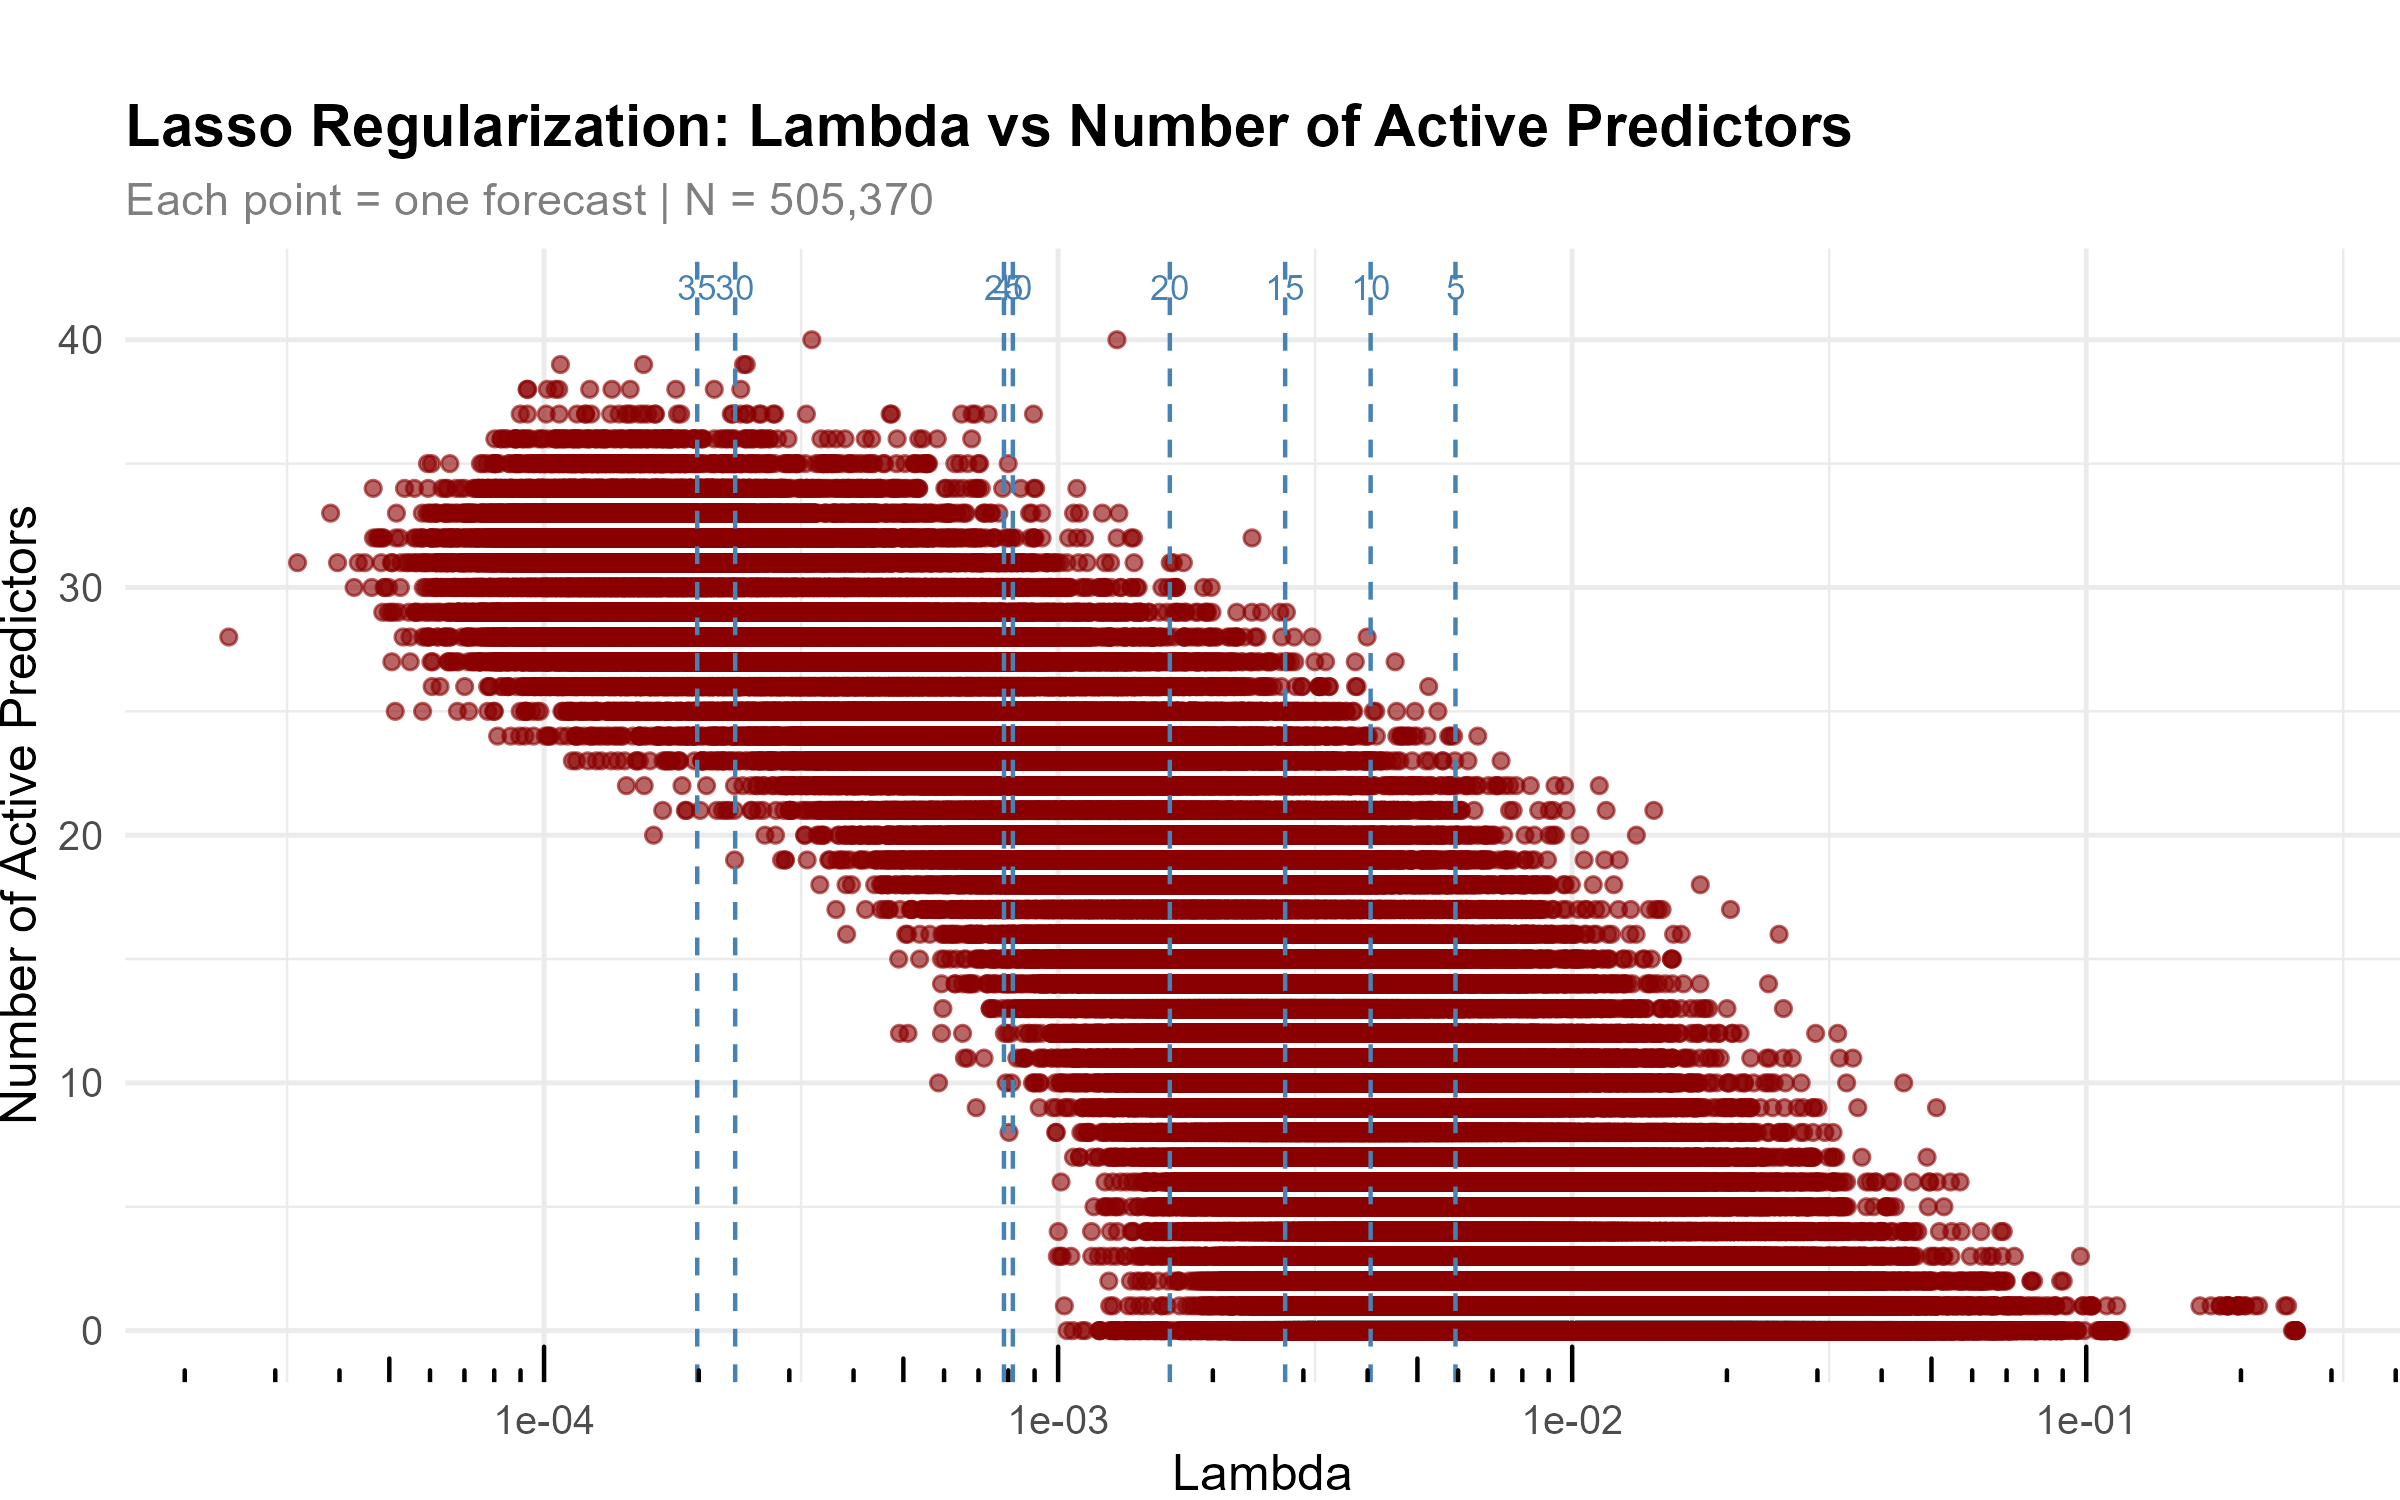
\includegraphics[width=0.45\textwidth]{lambdavspredictors.png} 
    \caption{Number of predictors selected by LASSO as a function of $\lambda$.}
    \label{fig:var_selec} % Label for referencing
\end{figure}

Next, we compare the out-of-sample performance of the LASSO forecasts with a simple benchmark that always predicts the in-sample mean. Figure~\ref{fig:r2_oos_lasso} shows that, on average, the LASSO forecasts underperform this historical mean benchmark.

\begin{figure}[h!] % h! means "place here, if possible"
    \centering
    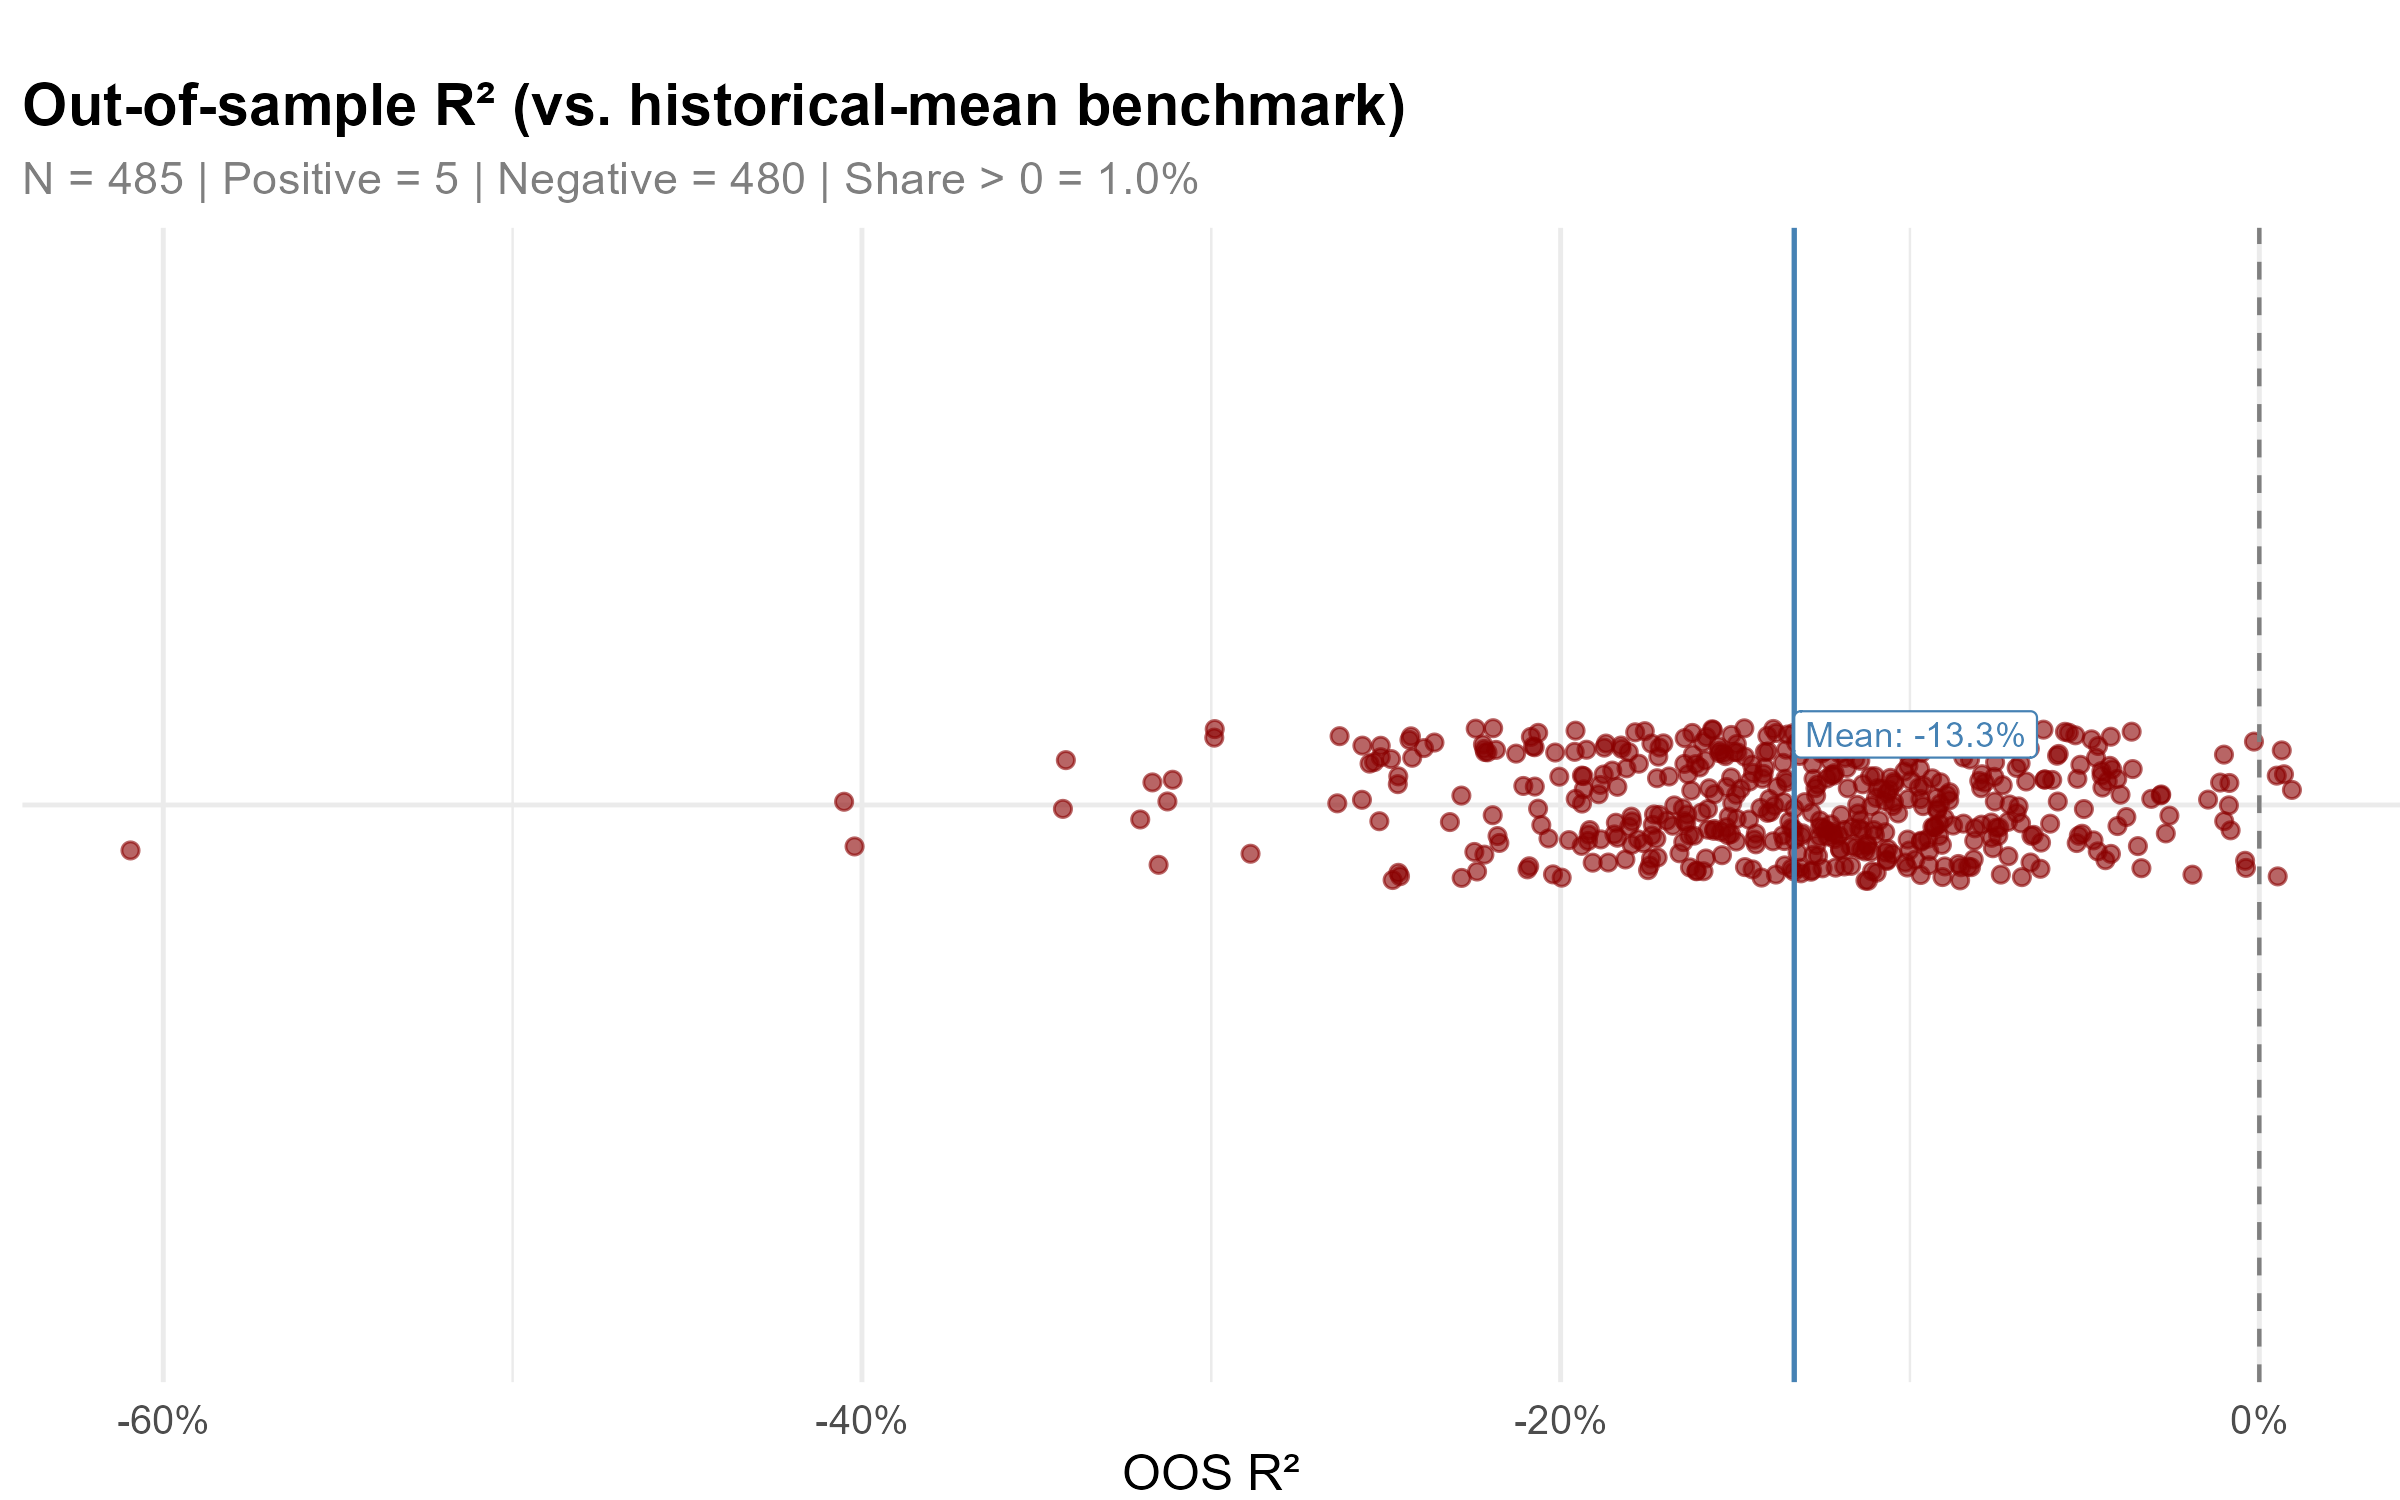
\includegraphics[width=0.45\textwidth]{r2_oss.png} 
    \caption{Out-of-sample $R^2$ of LASSO forecasts relative to the mean benchmark.}
    \label{fig:r2_oos_lasso} % Label for referencing
\end{figure}

In line with \cite{chinco2019sparse}, we continue by exploring whether augmenting a standard benchmark model with the predictors selected by the LASSO improves out-of-sample fit. We construct an AR(3) benchmark forecast for each stock and then expand it by including the LASSO-selected variables. If this combined model delivers a statistically significant increase in $R^2_{oos}$, we interpret it as evidence that the LASSO is capturing information not already contained in the benchmark model.

\begin{figure}[h!] % h! means "place here, if possible"
    \centering
    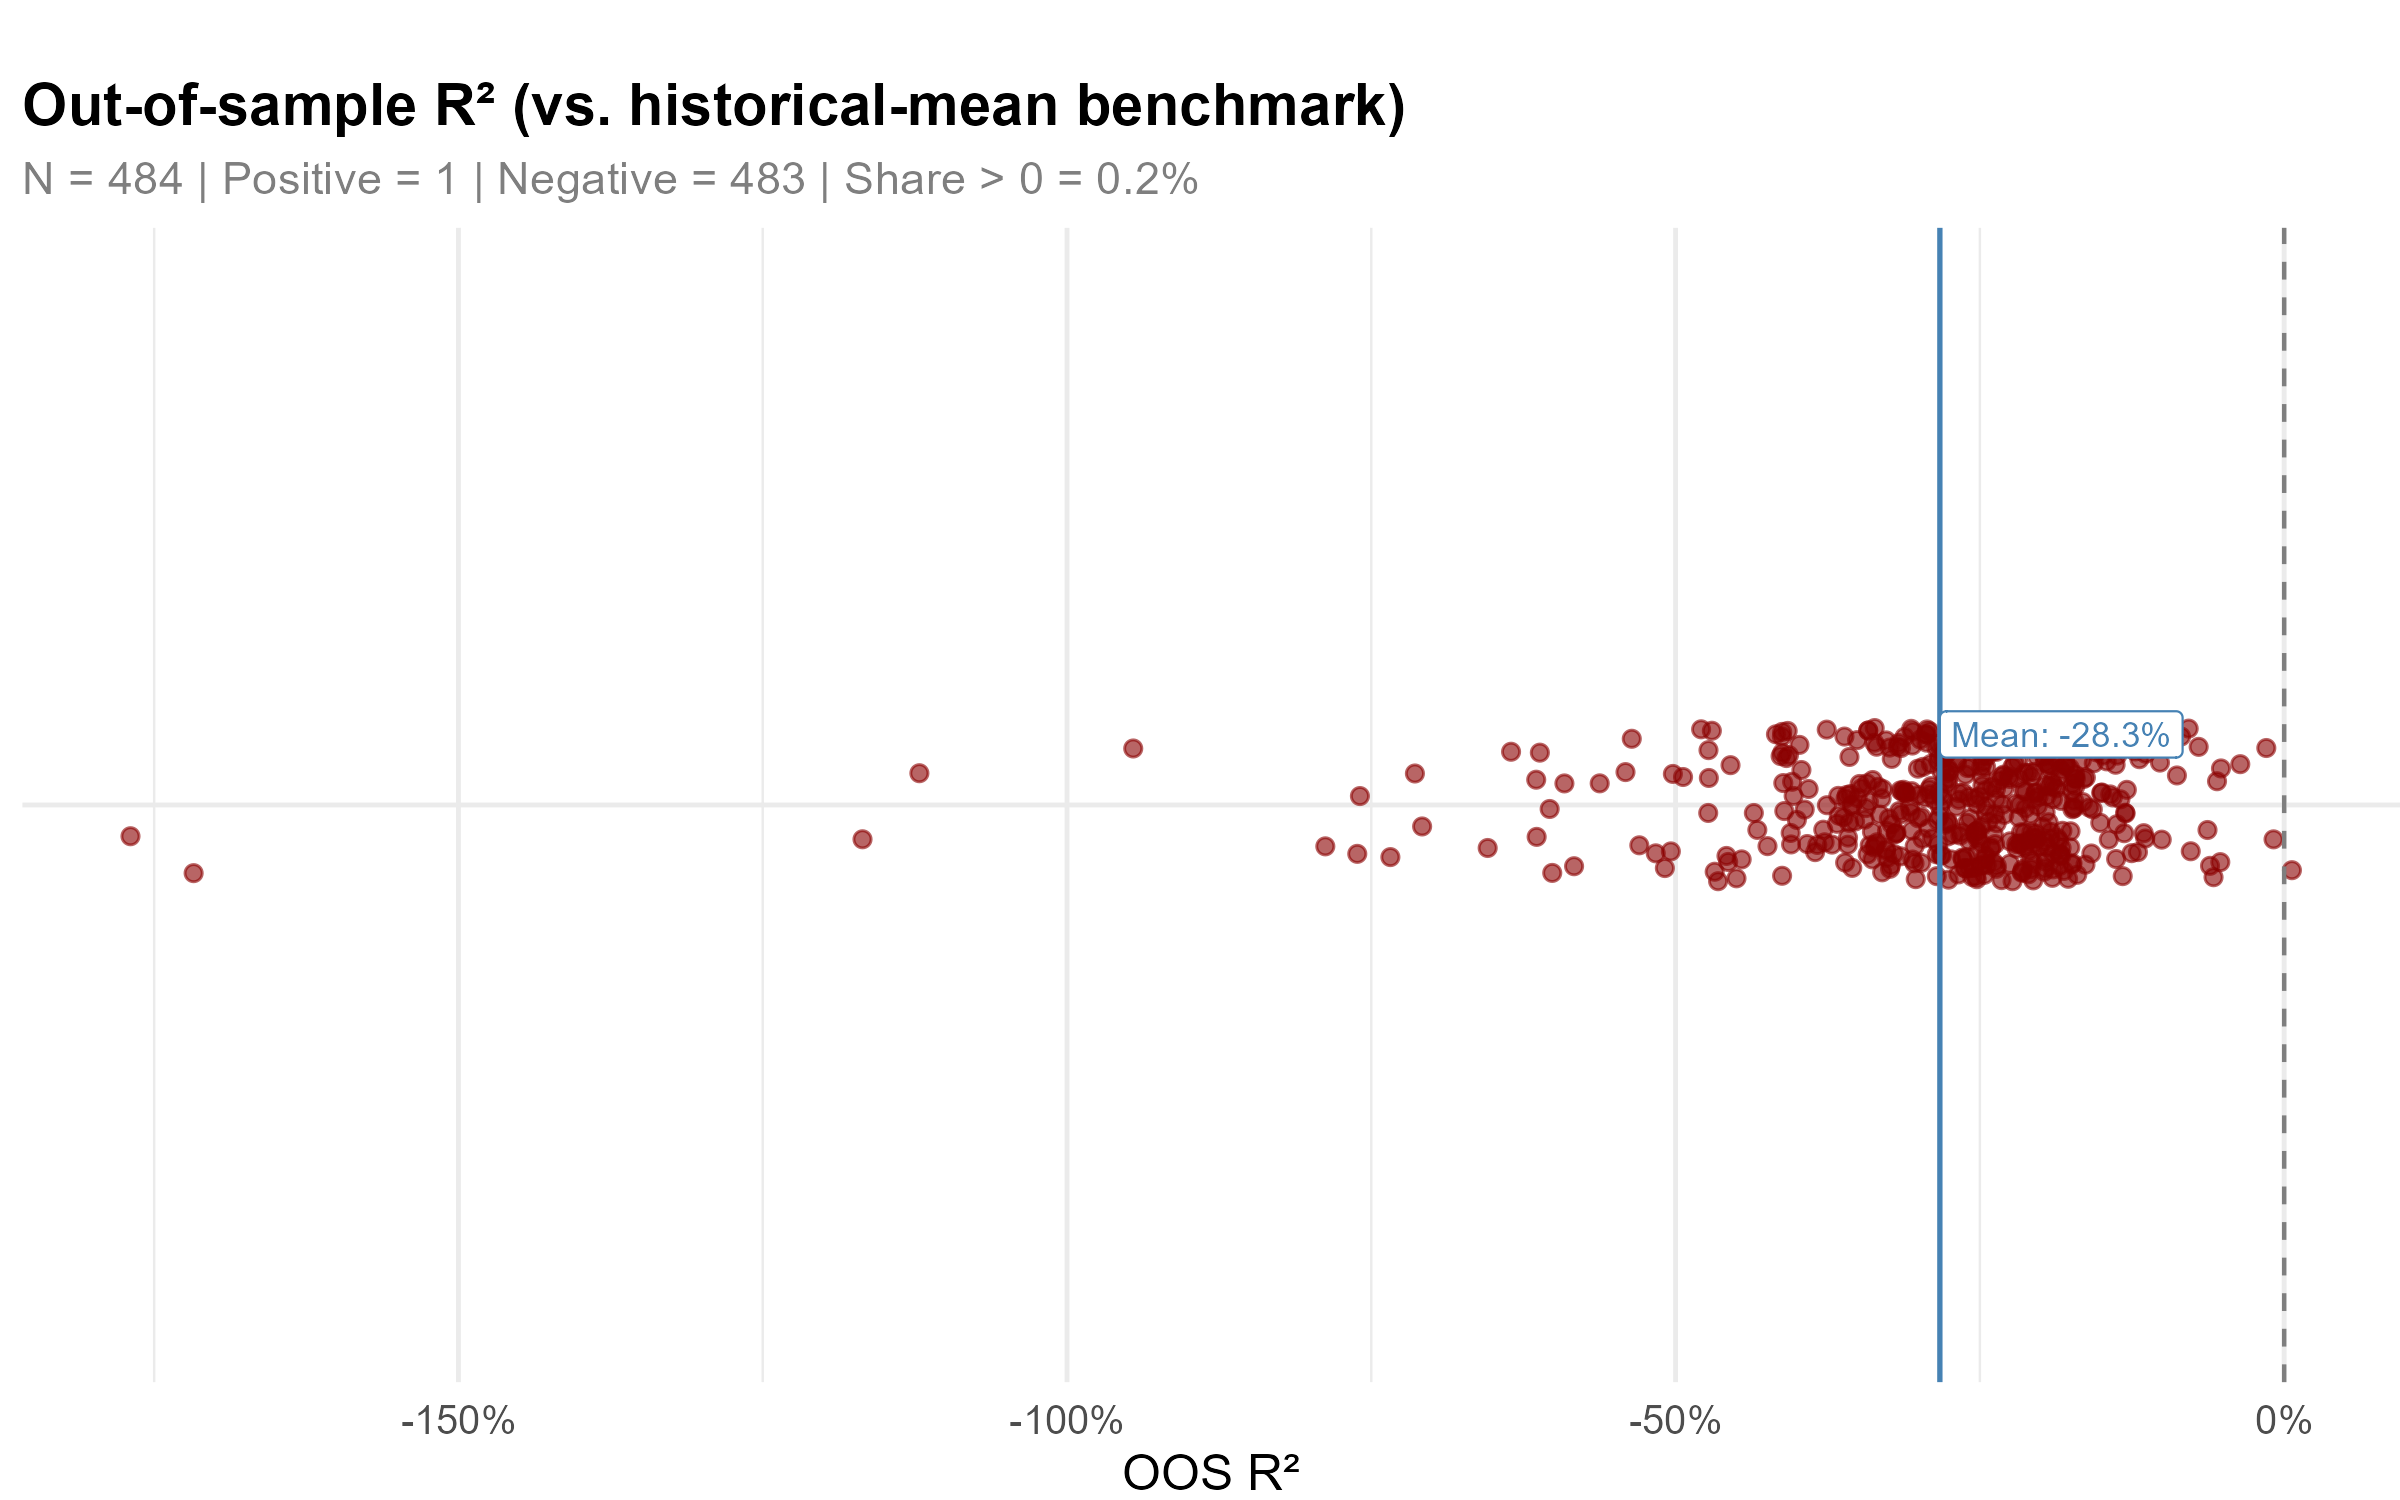
\includegraphics[width=0.45\textwidth]{r2_oss_ar3.png} 
    \caption{Out-of-sample $R^2$ of the AR(3) benchmark model.}
    \label{fig:r2_oos_benchmark} % Label for referencing
\end{figure}

% \begin{figure}[h!] % h! means "place here, if possible"
%     \centering
%     \includegraphics[width=0.45\textwidth]{} 
%     \caption{Out-of-sample $R^2$ of the AR(3) benchmark augmented with LASSO predictors.}
%     \label{fig:r2_oos_benchmar_lasso} % Label for referencing
% \end{figure}

Figure~\ref{fig:r2_oos_benchmark} shows that the benchmark model alone achieves, on average, a much lower $R^2_{oos}$ than the LASSO specification. When the benchmark is augmented with the variables selected by LASSO, $R^2_{oos}$ rises significantly. This indicates that our variable selection method captures information from the cross-section of stock returns and news attention that the AR(3) benchmark does not.

Finally, we analyze the time-series properties of the predictors selected by LASSO. Figure~\ref{persistence} shows the daily share of selected predictors that exhibit persistence. Persistence is assessed by estimating an AR(1) model for each selected predictor, using the same 30-day rolling window applied in the LASSO estimation. A predictor is classified as persistent if its autoregressive coefficient is statistically significant at the 5\% level. On average, about 8\% of predictors on a given day are persistent. This share varies considerably over time and tends to increase during periods of elevated market volatility (e.g., the COVID-19 crash).

\begin{figure}[h!] % h! means "place here, if possible"
    \centering
    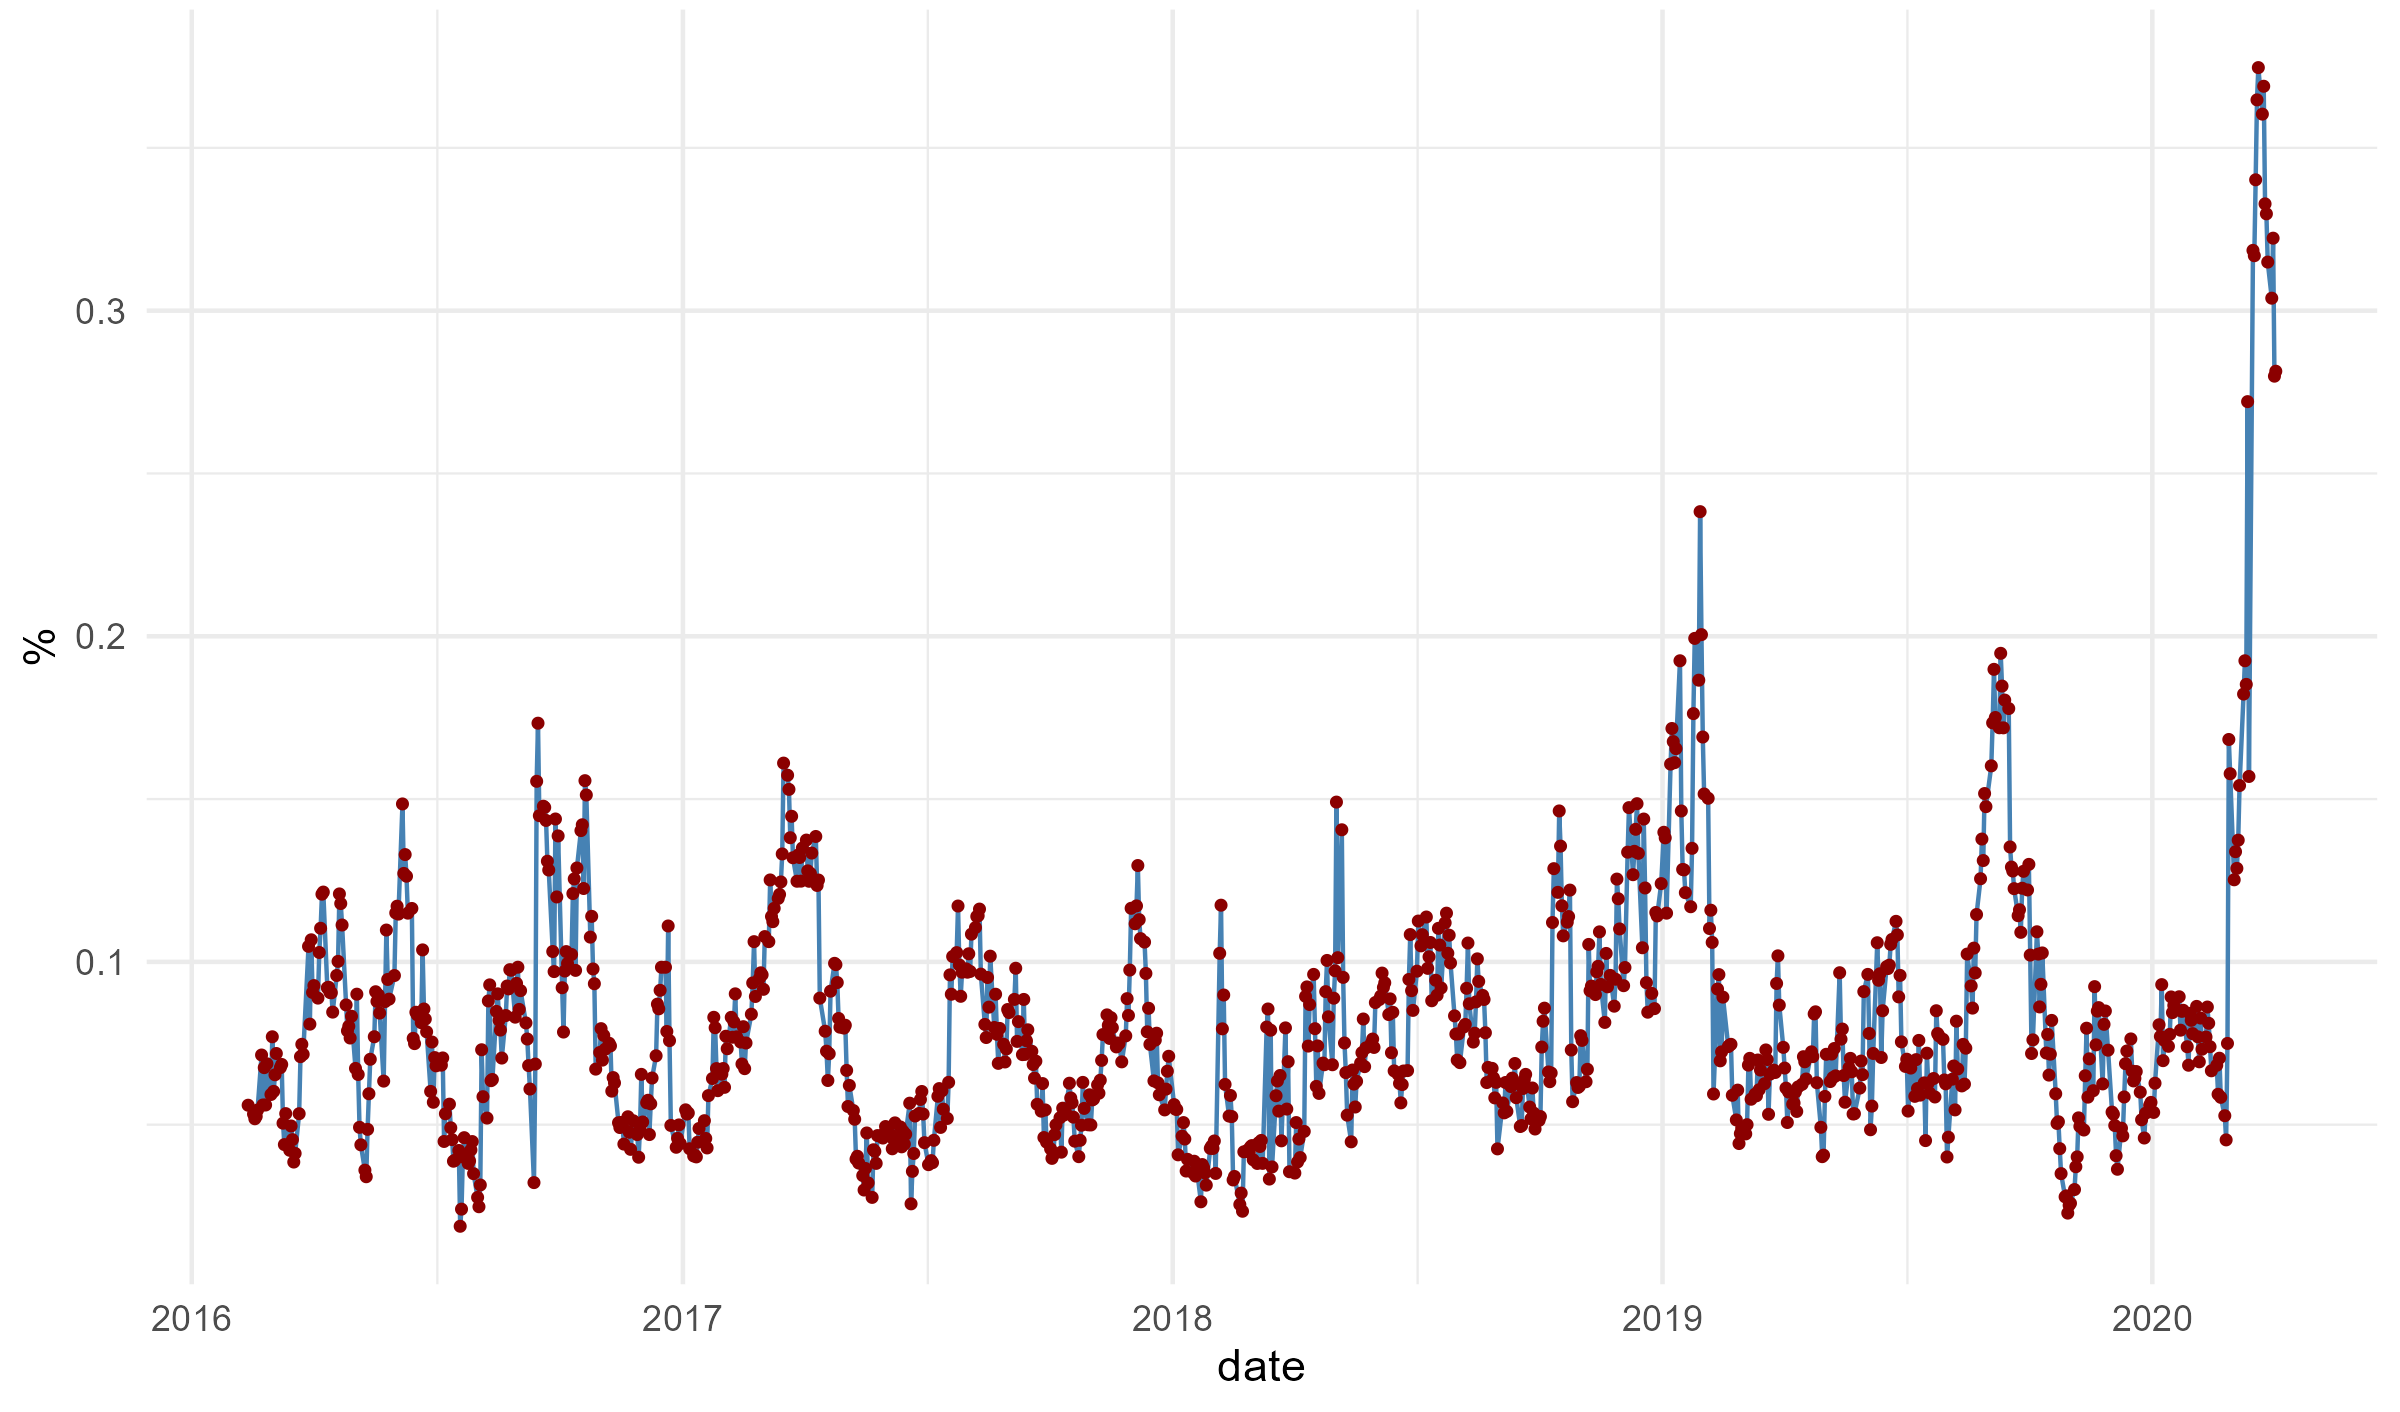
\includegraphics[width=0.45\textwidth]{dately_share_plot.png} 
    \caption{Daily share of LASSO-selected predictors classified as persistent.}
    \label{fig:persistence} % Label for referencing
\end{figure}
\printbibliography


\end{document}
